\documentclass[12pt]{iopart}

\usepackage{iopams}

\makeatletter
\@namedef{ver@amsmath.sty}{}
\makeatother

\usepackage{siunitx}
\usepackage{isotope}
\usepackage{fixltx2e}
\usepackage{booktabs}
\usepackage{xcolor}
\usepackage{multirow}
\usepackage{url}
\usepackage{graphicx}
\usepackage{tikz}
\usepackage{tabularx}
\usepackage[all=normal,bibbreaks=tight,floats=tight,mathspacing=tight,wordspacing=tight]{savetrees}

\providecommand{\keywords}[1]{\textbf{\textit{Index terms---}} #1}
\newcommand{\DDO}{D\textsubscript{2}O}
\definecolor{datacolor}{RGB}{72,36,117}

\graphicspath{{./fig_final_report/}{./fig/}}

\newcommand{\surrogateplot}[6]{
\begin{tikzpicture}
	\node[anchor=south west,inner sep=0] at (0,0){\includegraphics[width=\textwidth]{#1}};
	\draw[black,fill=white,line
		width=0.05mm,align=right,font=\fontsize{5.5}{6.5}\selectfont]
		(0.42,#6) rectangle
		(2.55,2.7) node[pos=.5] {
			\\[0.1ex]
			$\mathrm{MAE} = \num{#2}$\\
			$S = \num{#3}$\\
			$R^2 = \num{#4}$\\
			$R^2_{\text{adj.}} = \num{#5}$
		};
	\draw[black,fill=white,line
		width=0.05mm,align=left,font=\fontsize{5.5}{7.5}\selectfont]
		(2.02,1.3) rectangle
		(4.3,0.38) node[pos=.5] {
			{\color{red}
			\leavevmode\leaders\hrule height 0.7ex
			depth\dimexpr0.4pt-0.7ex\hskip3pt\kern0pt
			\hskip1pt
			\leavevmode\leaders\hrule height 0.7ex
			depth\dimexpr0.4pt-0.7ex\hskip3pt\kern0pt
			} Ideal model\\
			{\leavevmode\leaders\hrule height 0.7ex
			depth\dimexpr0.4pt-0.7ex\hskip3pt\kern0pt
			\hskip1pt
			\leavevmode\leaders\hrule height 0.7ex
			depth\dimexpr0.4pt-0.7ex\hskip3pt\kern0pt
			} Trained model\\
			\hskip3pt\raisebox{0.25ex}{\scalebox{0.75}{\color{datacolor}\textbullet}}\hskip4pt Data
		};
\end{tikzpicture}}

\begin{document}

%%%%%%%%%%%%%%%%%%%%%%%%%%%%%%%%%%%%%%%%%%%%%%%%%%%%%%%%%%%%%%%%%%%%%%%%%%%%%%%
% FRONT MATTER
%%%%%%%%%%%%%%%%%%%%%%%%%%%%%%%%%%%%%%%%%%%%%%%%%%%%%%%%%%%%%%%%%%%%%%%%%%%%%%%

\title[Fast Regression of the Tritium Breeding Ratio in Fusion Reactors]{Fast Regression of the
Tritium Breeding Ratio in Fusion Reactors}

\author{P~Mánek$^{1,2}$, G~Van Goffrier$^1$, V~Gopakumar$^3$, N~Nikolaou$^1$, J~Shimwell$^3$ and I~Waldmann$^1$}

\address{$^1$ Department of Physics and Astronomy, University College London, Gower Street, London WC1E~6BT, UK}
\address{$^2$ Institute of Experimental and Applied Physics, Czech Technical University, Husova 240/5, Prague 110~00, Czech Republic}
\address{$^3$ UK Atomic Energy Authority, Culham Science Centre, OX14~3DB Abingdon, UK}

\eads{\mailto{petr.manek.19@ucl.ac.uk}, \mailto{graham.vangoffrier.19@ucl.ac.uk}}

\begin{abstract}
	The tritium breeding ratio (TBR) is an essential quantity for the design of
	modern and next-generation D-T fueled nuclear fusion reactors. Representing the
	ratio between tritium fuel generated in breeding blankets and fuel consumed
	during reactor runtime, the TBR depends on reactor geometry and material
	properties in a complex manner. In this work, we explored the
	training of surrogate models to produce a cheap but high-quality approximation
	for a Monte Carlo TBR model in use at the UK Atomic Energy Authority. We
	investigated possibilities for dimensional reduction of its feature space, reviewed
	9~families of surrogate models for potential
	applicability, and performed hyperparameter optimisation. Here we present the
	performance and scaling properties of these
	models, the fastest of which, an artificial neural network,
	demonstrated~$R^2=\num{0.985}$ and a mean
	prediction time of~$\SI{0.898}{\micro\second}$, representing a relative speedup of $8\cdot 10^6$
	with respect to the expensive MC model. We further present a novel adaptive
	sampling algorithm, Quality-Adaptive Surrogate Sampling, capable
	of interfacing with any of the individually studied surrogates. Our preliminary
	testing on a toy TBR theory has demonstrated the efficacy of this algorithm for
	accelerating the surrogate modelling process.
\end{abstract}

\keywords{machine learning, surrogate model, regression, fast approximation,
Monte Carlo simulation, OpenMC, Paramak, tritium breeding, adaptive sampling}
\submitto{\NF}
\maketitle
\ioptwocol

%%%%%%%%%%%%%%%%%%%%%%%%%%%%%%%%%%%%%%%%%%%%%%%%%%%%%%%%%%%%%%%%%%%%%%%%%%%%%%%
% MAIN MATTER
%%%%%%%%%%%%%%%%%%%%%%%%%%%%%%%%%%%%%%%%%%%%%%%%%%%%%%%%%%%%%%%%%%%%%%%%%%%%%%%

\section{Introduction}
\label{sec:introduction}
%TODO: make all more concise, bullet points

\begin{frame}
	\frametitle{Project Background}
	Nuclear fusion -- the energy of the future!
    \vspace{10pt}
	\begin{itemize}
	    \item Must produce and contain an extremely hot and dense plasma
	    \begin{itemize}
		    \item Magnetic Confinement Fusion (MCF): toroidal circulation
		    \item Inertial Confinement Fusion (ICF): spherical compression
		\end{itemize}
		\vspace{10pt}
		\item Modern designs require enriched Hydrogen fuel of two varieties:
	    \begin{itemize}
		    \item Deuterium ($^2$H) -- abundant in naturally-sourced water.
		    \item Tritium ($^3$H) -- extremely rare, but can be produced \textit{in-reactor}.
		\end{itemize}
	\end{itemize}
	\vspace{10pt}
	\centering{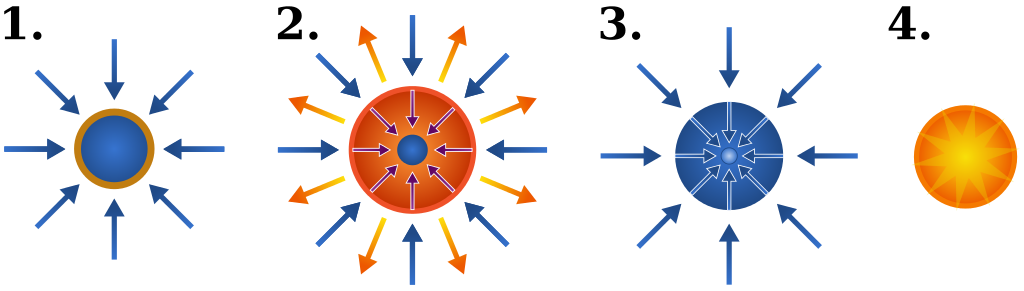
\includegraphics[height=3cm]{icf_diagram}}
\end{frame}

\begin{frame}
	\frametitle{Problem Description}
	Tritium breeding blankets convert neutron radiation to tritium fuel:
	\begin{align*}
		\isotope[1][0]{n} + \isotope[6][3]{Li} \rightarrow \isotope[3][1]{H} +
		\isotope[4][2]{He}
		\qquad\qquad
		\isotope[1][0]{n} + \isotope[7][3]{Li} \rightarrow \isotope[3][1]{H} +
		\isotope[4][2]{He} + \isotope[1][0]{n}
	\end{align*}
	Tritium breeding ratio (TBR) = fuel bred / fuel consumed
	
	\begin{itemize}
	    \item Depends on numerous geometric and material parameters.
	    \item Evaluated precisely by OpenMC neutronics simulation \textit{Paramak}, but is computationally expensive. 
	\end{itemize}
	
	\vspace{15pt}
	
	\begin{block}{Our Challenge:}
		\begin{center}
			Produce a fast TBR function that strongly approximates Paramak, making use of the latest in surrogate modelling techniques.
		\end{center}
	\end{block}
\end{frame}

\begin{frame}
	\frametitle{Data Generation}
	We produced training and test datasets by uniform random sampling over the 7
	discrete and 11 continuous parameters of Paramak.

	\begin{columns}[T]
		\column{0.34\textwidth}

		\vspace{5pt}

		Paramak was deployed on UCL's Hypatia cluster:
		\begin{itemize}
		\item Generated 1M samples.
		\item 27 days of runtime.
		\end{itemize}

		\vspace{5pt}

		2~classes of runs:
		\begin{itemize}
		\item All parameters free.
		\item Discrete fixed, continuous free.
		\end{itemize}

		\vspace{5pt}

		{\footnotesize
		Groups of fractions marked\textsuperscript{\textdagger\textdaggerdbl} are required to sum to 1.
		}

		\column{0.62\textwidth}
		\vspace{5pt}

		{\fontsize{8pt}{8pt}\selectfont
		\setlength\tabcolsep{3pt}
		\begin{tabular}{l|ll}
		\toprule
		{} & Parameter name & Domain\\
		\midrule
		\parbox[t]{2mm}{\hspace{-2pt}\multirow{12}{*}{\rotatebox[origin=c]{90}{Blanket}}}
		   & Breeder fraction\textsuperscript{\textdagger} & $[0,1]$\\
		   & Breeder \isotope[6]{Li} enrichment fraction & $[0,1]$\\
		   & Breeder material & $\{\text{Li}_2\text{TiO}_3, \text{Li}_4\text{SiO}_4\}$\\
		   & Breeder packing fraction & $[0,1]$\\
		   & Coolant fraction\textsuperscript{\textdagger} & $[0,1]$\\
		   & Coolant material & $\{\text{D}_2\text{O}, \text{H}_2\text{O}, \text{He}\}$\\
		   & Multiplier fraction\textsuperscript{\textdagger} & $[0,1]$\\
		   & Multiplier material & $\{\text{Be}, \text{Be}_{12}\text{Ti}\}$\\
		   & Multiplier packing fraction & $[0,1]$\\
		   & Structural fraction\textsuperscript{\textdagger} & $[0,1]$\\
		   & Structural material & $\{\text{SiC}, \text{eurofer}\}$\\
		   & Thickness & $[0,500]$\\
		\midrule
		\parbox[t]{2mm}{\hspace{-2pt}\multirow{6}{*}{\rotatebox[origin=c]{90}{First wall}}}
		   & Armour fraction\textsuperscript{\textdaggerdbl} & $[0,1]$\\
		   & Coolant fraction\textsuperscript{\textdaggerdbl} & $[0,1]$\\
		   & Coolant material & $\{\text{D}_2\text{O}, \text{H}_2\text{O}, \text{He}\}$\\
		   & Structural fraction\textsuperscript{\textdaggerdbl} & $[0,1]$\\
		   & Structural material & $\{\text{SiC}, \text{eurofer}\}$\\
		   & Thickness & $[0,20]$\\
		\bottomrule
		\end{tabular}
		}

    \end{columns}
\end{frame}

%\begin{frame}
%	\frametitle{Dimensionality Reduction}
%	\begin{itemize}
%		\item % TODO
%	\end{itemize}
%\end{frame}

\begin{frame}
	\frametitle{Methodology}
		Conventional regression task -- search for a cheap surrogate $\hat{f}(x)$ that
		minimizes dissimilarity with an expensive function $f(x)$:

		\begin{itemize}
			\item
				Regression performance: mean absolute error, $\sigma$ of
				error, $R^2$, $R^2_\text{adj.}$
			\item
				Computational complexity:
				training \& prediction time / sample
		\end{itemize}

		\vspace{2em}

		2 approaches for surrogate training:
		\begin{enumerate}
			\item
				Decoupled -- trains models from previously sampled
				datapoints.
			\item
				Adaptive -- repeats sampling \& model training, increases
				sampling density in low-performance regions.
		\end{enumerate}
\end{frame}



\section{Methodology}
\label{sec:methodology}
Labeling the expensive MC TBR model $f(x)$, a surrogate is a mapping
$\hat{f}(x)$ such that $f(x)$ and $\hat{f}(x)$ minimise a selected dissimilarity
metric. In order to be considered \textit{viable}, $\hat{f}(x)$ is required to
achieve expected evaluation time lower than that of~$f(x)$. In this work, we
consider 2~methods of producing viable surrogates: (1)~a conventional decoupled
approach, which evaluates $f(x)$ on a set of randomly sampled points and
trains surrogates in a supervised scheme, and (2)~an adaptive approach, which attempts to
compensate for localised regression performance insuficiencies by interleaving
multiple epochs of sampling and training.

\begin{table}[t]
	\setlength\tabcolsep{2pt}
	\renewcommand{\arraystretch}{0.95}
	\caption{\label{tbl:surrogates}Considered surrogate model families, their
		selected abbreviations and implementations. $\mathcal{H}$~denotes the
		set of hyperparameters.}
	\begin{indented}
	\item[]
		\begin{tabular}{lllr}
		\toprule
		Surrogate family & Abbr. & Impl. & $|\mathcal{H}|$ \\
		\midrule
		Support vector machines~\cite{fan2008liblinear}	& SVM & SciKit~\cite{scikit-learn} & 3 \\
		Gradient boosted trees~\cite{friedman2001greedy,friedman1999stochastic,hastie2009elements}	& GBT & SciKit & 11 \\
		Extremely randomised trees~\cite{geurts2006extremely}	& ERT & SciKit & 7 \\
		AdaBoosted decision trees$^\text{a}$~\cite{drucker1997improving}	& ABT & SciKit & 3 \\
		Gaussian process regression~\cite{williams2006gaussian}	& GPR & SciKit & 2 \\
		$k$ nearest neighbours	& KNN & SciKit & 3 \\
		Artificial neural networks	& ANN & Keras~\cite{chollet2015keras} & 2 \\
		Inverse distance weighing~\cite{shepard1968two} & IDW & SMT~\cite{SMT2019} & 1 \\
		Radial basis functions & RBF & SMT & 3 \\
		\bottomrule
		\end{tabular}\\%
		{\footnotesize $^\text{a}$Note that ABTs can be viewed as a subclass of GBTs.}
	\end{indented}
\end{table}

\begin{table*}[t]
	\renewcommand{\arraystretch}{0.95}
	\caption{\label{tbl:metrics}Metrics recorded in experiments. In
	formulations, we work with a training set of size $N_0$ and a test set of
size $N$, values $y^{(i)}=f(x^{(i)})$ and $\hat{y}^{(i)}=\hat{f}(x^{(i)})$
denote images of the $i$th testing sample in the MC TBR model and the surrogate
respectively. The mean $\overline{y}=N^{-1}\sum_{i=1}^N y^{(i)}$ and $P$ is the
number of input features.}
	\begin{indented}
	\item[]
		\begin{tabularx}{\textwidth}{Xrl}
		\toprule
		Regression performance metrics& Notation	& Mathematical formulation\\
		\midrule
		Mean absolute error	& MAE & $N^{-1}\sum_{i=1}^N |y^{(i)}-\hat{y}^{(i)}|$ \\
		Standard deviation of error & $S$	& $\text{StdDev}_{i=1}^N\left\{ |y^{(i)} -
		\hat{y}^{(i)}| \right\} $ \\
			Coefficient of determination & $R^2$	& $1-\sum_{i=1}^N
			\left(y^{(i)}-\hat{y}^{(i)} \right)^2\left[\sum_{i=1}^N \left(
			y^{(i)}-\overline{y} \right)^2\right]^{-1} $ \\
			Adjusted $R^2$ & $R^2_\text{adj.}$	& $1-(1-R^2)(N-1)(N-P-1)^{-1}$ \\
		\midrule
		Computational complexity metrics	& {}	& {} \\
		\midrule
		Mean training time & $\overline{t}_{\text{trn.}}$	& $(\text{wall training time of
		$\hat{f}(x)$})N_0^{-1}$  \\
			Mean prediction time & $\overline{t}_{\text{pred.}}$	& $(\text{wall prediction time of
			$\hat{f}(x)$})N^{-1}$ \\
				Relative speedup & $\omega$	& $(\text{wall evaluation$^\text{b}$ time of $f(x)$})
				(N\overline{t}_{\text{pred.}})^{-1}$ \\
		\bottomrule
		\end{tabularx}\\%
		{\footnotesize $^\text{b}$This corresponds to evaluation of Paramak
		 on all points of the test set. In surrogates, the equivalent
		time period is referred to as ``prediction time.''}
	\end{indented}
\end{table*}

For both methods, we selected state-of-the-art regression algorithms to perform
surrogate training on sampled point sets. Listed in~\Tref{tbl:surrogates}, these
implementations define 9~surrogate families that are later reviewed in~\Sref{sec:results}.
We note that each presented algorithm defines hyperparameters that may influence its
performance. Their problem-specific optimal values are searched within the scope
of this work, in particular in Experiments~1 \&~2 that are outlined
in~\Sref{sec:experiment-methodology}.

To compare the quality of the produced surrogates, we define a number of metrics listed
in~\Tref{tbl:metrics}. For regression performance analysis, we include a
selection of absolute metrics to assess the models' approximation capability and set
practical bounds on the expected uncertainty of their predictions. In addition, we also track
relative measures that are better-suited for comparison between this work and others as
they are invariant with respect to the selected domain and image space.
For analysis of computational complexity, surrogates are assessed in terms of wall
time (captured by the Python~3 \texttt{time} package). This is motivated by common practical use
cases of our work, where models are trained and used as drop-in replacements for
Paramak. All times reported (training, test, evaluation) are
normalized by the corresponding dataset size, i.e.~correspond to ``time to
process a single datapoint.''

Even though some surrogates support acceleration by means of parallelisation, we
used non-parallelized implementations. The only exception to this are ANNs,
which require a considerable amount of processing power for training on
conventional CPU architectures. Lastly, to prevent undesirable bias by training
set selection, all reported metrics are obtained via 5-fold cross-validation.
In this setting, a sample set is uniformly divided into 5 disjoint folds, each of which
is used as a test set for models trained on the remaining 4. Having repeated the
same experiment for each division, the overall value of individual metrics is
reported in terms of their mean and standard deviation over all folds.



\subsection{Decoupled Approach}\label{sec:experiment-methodology}

Experiments related to the decoupled approach are organised in 4~parts,
further described in this section. In summary, we aim to optimise the hyperparameters of
each surrogate family separately and later use the best found results to compare surrogate
families among themselves.

The objective of Experiment~1 is to simplify the regression task for
surrogates prone to suboptimal performance in discontinuous spaces.
To this end, training points are filtered to a single selected discrete feature
assignment, and surrogates are trained only on the remaining continuous features.
This is repeated several times to explore variances in behaviour,
particularly in 4~distinct assignments that are obtained by setting blanket and
first wall coolant materials to one
of:~$\{\text{H\textsubscript{2}O},\isotope{He}\}$.
Experiment~2 conventionally measures surrogate performance on the full feature
space without any parameter restrictions. In both experiments, hyperparameter tuning is
facilitated by Bayesian optimisation~\cite{movckus1975bayesian}, where we select the
hyperparameter configuration that produces the model that maximises $R^2$. The
process is terminated after 1000~iterations or 2~days, whichever condition is satisfied first.
The results of Experiments~1 \&~2 are depicted
in Figures~\ref{fig:exp1-time-vs-reg} \&~\ref{fig:exp2-time-vs-reg}
respectively, and described in~\Sref{sec:res-exp12}.

In Experiment~3, the 20~best-performing hyperparameter configurations
per each model family are used to train surrogates on sets of various sizes to
investigate their scaling properties. In particular, we consider sets of
sizes~$\{1,2,5,10,12,15,20\}$ in thousands of samples to better characterize the
relationship of each family between sample count and the metrics of interest
listed in~\Tref{tbl:metrics}.
The results of this experiment are shown in~\Fref{fig:scaling} and discussed
in~\Sref{sec:res-exp3}.

Finally, Experiment~4 aims
to produce surrogates suitable for practical use by retraining selected
well-scaling instances on large training sets in order to satisfy the goals of this work.
The results of this process are displayed in~\Fref{fig:reg-performance} and
in~\Tref{tbl:exp4-detailed-results}, and summarized in~\Sref{sec:res-exp4}.


\subsection{Adaptive Approach}\label{sec:adaptive}

Adaptive sampling techniques appear frequently in the literature and have been specialised for surrogate modelling, where precision is implicitly limited by the quantity of training samples which are available from the expensive model. Garud's~\cite{Garud2016} ``Smart Sampling Algorithm'' achieved notable success by incorporating surrogate quality and
crowding distance scoring to identify optimal new samples, but was only tested
on a single-parameter domain. We theorised that a nondeterministic sample
generation approach, built around Markov Chain Monte Carlo methods (MCMC), would
fare better for high-dimensional models by more thoroughly exploring all local
optima in the feature space. MCMC produces each sample points according to a shared proposal
distribution from the prior point. These sample points will converge to a desired posterior
distribution, so long as the acceptance probability meets certain statistical criteria (see~\cite{Zhou2018} for a review).

\begin{figure}
	\centering
	\hspace*{-5pt}\includegraphics[width=1.28\linewidth]{fig4_qassplan.png}
	\caption{\label{fig:qassplan}Schematic of QASS algorithm}
\end{figure}

Many researchers have embedded surrogate methods into MCMC strategies for
parameter optimisation~\cite{Zhang2020,Gong2017}, in particular the ASMO-PODE
algorithm~\cite{Ginting2011} which makes use of MCMC-based adaptive sampling. Our approach draws inspiration from ASMO-PODE, but instead uses MCMC to generate samples
which increase surrogate precision throughout the entire parameter space.

We designed the Quality-Adaptive Surrogate Sampling algorithm (QASS, \Fref{fig:qassplan}) to iteratively increment the training/test set with sample
points which maximise surrogate error and minimise a crowding distance metric
(CDM)~\cite{Solonen2012} in feature space. On each iteration following an initial training of the surrogate on $N$ uniformly random samples, the surrogate was trained and absolute error calculated. MCMC was then performed on the error function generated by performing nearest-neighbor interpolation on these test error points. The resultant samples were culled by $50\%$ according to the CDM, and then the $n$ highest-error candidates were selected for reintegration with the training/test set, beginning another training epoch. Validation was also performed during each iteration on independent, uniformly-random sample sets.


\section{Results}
\label{sec:results}
\subsection{Decoupled Approach}
\label{sec:modelres}

\subsubsection{Hyperparameter Tuning}

The results displayed in~\Fref{fig:exp1-time-vs-reg} indicate that in the first,
simplified case GBTs clearly appear to be the most accurate as
well as the fastest surrogate family in terms of mean prediction time. Following
that, we note that ERTs, SVMs and ANNs also achieved satisfactory results with respect to both examined metrics.
While the remainder of tested surrogate families does not exhibit prohibitive
complexity, its regression performance falls below average.

\begin{figure}
	\centering
	\includegraphics[width=0.9\linewidth]{exp1_slice0}
	\includegraphics[width=0.9\linewidth]{exp1_slice1}
	\includegraphics[width=0.9\linewidth]{exp1_slice2}
	\caption{\label{fig:exp1-time-vs-reg}20~best-performing surrogates per each considered family, plotted in
		terms of complexity (as~$\overline{t}_{\text{pred.}}$) and regression
		performance (as~$R^2$) with 3~selected discrete feature assignments.}
\end{figure}

Comparing these results with those of the second, unrestricted experiment (shown
in~\Fref{fig:exp2-time-vs-reg}), we observe that many surrogate families
consistently underperform. The least
affected models appear to be GBTs, ANNs and ERTs, which are known to be capable of capturing relationships
involving mixed feature types that were deliberately withheld in the first
experiment. With only negligible differences, the first two of these families
appear to be tied for the best performance as well as the shortest prediction
time. We observe that ERTs and RBFs also
demonstrated satisfactory results, clearly outperforming the remaining surrogates in
terms of regression performance, and in some cases also in prediction time.

\begin{figure}
	\centering
	\includegraphics[width=0.9\linewidth]{exp2_time_vs_reg}
	\caption{\label{fig:exp2-time-vs-reg}Results of Experiment~2, plotted analogously
	to~\Fref{fig:exp1-time-vs-reg}.}
\end{figure}

Following both hyperparameter tuning experiments, we conclude that while domain
restrictions employed in the first case have proven effective in improving the
regression performance of some methods, their performance fluctuates considerably
depending on the selected slices. Furthermore, in all instances the best
results are achieved by families of surrogates that do not benefit from this
restriction (GBTs, ANNs, ERTs).


\subsubsection{Scaling Benchmark}

The results shown in~\Fref{fig:scaling} suggest that in terms of regression
performance the most accurate families from the previous experiments
consistently maintain their relative advantage over others, even as
more training points are introduced. While such families achieve nearly comparable
performance on the largest dataset, in the opposite case tree-based ensemble approaches
clearly outperform ANNs. This can be observed
particularly on sets of sizes up to~\num{6000}.

\begin{figure}
	\centering
	\includegraphics[width=0.9\linewidth]{scaling_metric_r2}
	\includegraphics[width=0.9\linewidth]{scaling_time_train}
	\includegraphics[width=0.9\linewidth]{scaling_time_pred}
	\caption{Results of the scaling benchmark displayed as a function of
	training set size. From top to bottom, regression performance (as $R^2$),
	mean training time and mean prediction time.}
	\label{fig:scaling}
\end{figure}

Consistent with our expectation, the shortest training times were achieved by
instance-based learning methods (KNN, IDW) that
are trained trivially at the expense of increased lookup complexity later during prediction.
Furthermore, we observe that the majority of tree-based ensemble algorithms also perform
and scale well, unlike RBFs and GPR which appear to behave superlinearly. We note that ANNs,
which are the only family to utilise parallelisation during training, show an
inverse scaling characteristic. We suspect that this effect may be caused
by a constant multi-threading overhead that dominates the training process
on relatively small sets.

Finally, all tested families with the exception of previously mentioned instance-based
models offer desirable prediction times. Analogous to previous experiments,
GBTs, ABTs and ANNs appear to be tied, as they not only exhibit
comparable times but also similar scaling slopes. Following those, we note a
clear hierarchy of ERTs, SVMs, GPR and RBFs, trailed by IDW and KNNs.


\subsubsection{Model Comparison}
In Experiment~4, we aim to create models that yield:
(a)~the best regression performance regardless
of other features, (b)~acceptable performance with the shortest mean
prediction time, or (c)~acceptable performance with the smallest training set.
To this end, we trained 8~surrogates that are presented in~\Fref{fig:reg-performance}
and~\Tref{tbl:exp4-detailed-results}.
Having selected ANNs, GBTs, ERTs, RBFs and SVMs based on the results of
Experiments~2 \&~3, we utilised the best-performing hyperparameters.
In pursuit of goal~(a), the best approximator (Model~1,
ANN) achieved~$R^2=\num{0.998}$ and mean prediction
time~$\overline{t}_{\text{pred.}}=\SI{1.124}{\micro\second}$. These correspond
to a standard error~$S=\num{0.013}$ and a relative speedup~$\omega=\num{6916416} \times$
with respect to the MC TBR evaluation baseline. Satisfying
goal~(b), the fastest model (Model~2, ANN) achieved~$R^2=\num{0.985}$,
$\overline{t}_{\text{pred.}}=\SI{0.898}{\micro\second}$, $S=\num{0.033}$
and~$\omega=\num{8659251} \times$.
While these surrogates
were trained on the entire available set of~\num{500000} datapoints, to satisfy
goal~(c) we also trained a more simplified model (Model~4, GBT)
that achieved~$R^2=\num{0.913}$,
$\overline{t}_{\text{pred.}}=\SI{6.125}{\micro\second}$, $S=\num{0.072}$ and $\omega=\num{1269777} \times$
with a set of size only~\num{10000}.

\begin{table*}
	\centering
	\sisetup{round-mode=places,round-precision=3,detect-weight=true,detect-family=true}
	\caption{\label{tbl:exp4-detailed-results}Results of Experiment~4. Here,
		average values and standard deviations are reported over 5~cross-validation folds,
		$|\mathcal{T}|$~denotes cross-validation set size ($\times 10^3$)
		and $\omega$ is a relative speedup with respect to
		$\overline{t}_{\text{eval.}}=\num{7.777049573054314} \pm
		\num{2.8103592103930337} \text{ s}$
		measured in the MC TBR model over~\num{500000} samples.
	The best-performing method(s) under each are highlighted in bold.}
	\setlength\tabcolsep{4pt}
	\begin{indented}
	\item[]
		\scriptsize
		\begin{tabular}{lrrrrrrrr}
		\toprule
		{} & {} & \multicolumn{4}{c}{Regression performance} &
		\multicolumn{3}{c}{Complexity}\\
		\cmidrule(lr){3-6}
		\cmidrule(lr){7-9}
		Model & $|\mathcal{T}|$ & MAE [TBR] & $S$ [TBR] & $R^2$ [rel.] & $R^2_{\text{adj.}}$ [rel.]
						& $\overline{t}_{\text{trn.}}$ [\si{\milli\second}] &
		$\overline{t}_{\text{pred.}}$ [\si{\milli\second}] & $\omega$ [rel.]\\
		\midrule
		
		1 (ANN)
						& $\num[round-precision=0]{500.0}$
						& {\bfseries $\num{0.008777} \pm \num{0.000269}$}
						& {\bfseries $\num{0.012512} \pm \num{0.000535}$}
						& {\bfseries $\num{0.997995} \pm \num{0.000150}$}
						& {\bfseries $\num{0.997995} \pm \num{0.000150}$}
						& $\num{3.658670} \pm \num{0.035377}$
						& {\bfseries $\num{0.001124} \pm \num{0.000062}$}
						& $\num{6916416} \times$
\\

		2 (ANN)
						& $\num[round-precision=0]{500.0}$
						& $\num{0.025271} \pm \num{0.000719}$
						& $\num{0.033191} \pm \num{0.001331}$
						& $\num{0.985065} \pm \num{0.001069}$
						& $\num{0.985061} \pm \num{0.001069}$
						& $\num{2.989270} \pm \num{0.026018}$
						& {\bfseries $\num{0.000898} \pm \num{0.000037}$}
						& {\bfseries $\num{8659251} \times$}
\\

		3 (GBT)
						& $\num[round-precision=0]{200.0}$
						& $\num{0.058242} \pm \num{0.000528}$
						& $\num{0.059233} \pm \num{0.000337}$
						& $\num{0.941086} \pm \num{0.000844}$
						& $\num{0.941046} \pm \num{0.000845}$
						& $\num{2.220903} \pm \num{0.010040}$
						& $\num{0.006647} \pm \num{0.000218}$
						& $\num{1169933} \times$
\\

		4 (GBT)
						& $\num[round-precision=0]{10.0}$
						& $\num{0.070804} \pm \num{0.001843}$
						& $\num{0.071597} \pm \num{0.003491}$
						& $\num{0.913014} \pm \num{0.006027}$
						& $\num{0.911823} \pm \num{0.006110}$
						& {\bfseries $\num{1.621323} \pm \num{0.007535}$}
						& $\num{0.006125} \pm \num{0.000291}$
						& $\num{1269777} \times$
\\

		5 (ERT)
						& $\num[round-precision=0]{200.0}$
						& $\num{0.051286} \pm \num{0.000288}$
						& $\num{0.056296} \pm \num{0.000486}$
						& $\num{0.950486} \pm \num{0.000738}$
						& $\num{0.950453} \pm \num{0.000739}$
						& $\num{2.634038} \pm \num{0.009780}$
						& $\num{0.214195} \pm \num{0.003631}$
						& $\num{36308} \times$
\\

		6 (ERT)
						& $\num[round-precision=0]{40.0}$
						& $\num{0.067868} \pm \num{0.000302}$
						& $\num{0.071722} \pm \num{0.000461}$
						& $\num{0.917489} \pm \num{0.001005}$
						& $\num{0.917210} \pm \num{0.001009}$
						& $\num{2.368460} \pm \num{0.005461}$
						& $\num{0.187990} \pm \num{0.008412}$
						& $\num{41370} \times$
\\

		7 (RBF)
						& $\num[round-precision=0]{50.0}$
						& $\num{0.068405} \pm \num{0.000813}$
						& $\num{0.076889} \pm \num{0.001908}$
						& $\num{0.909963} \pm \num{0.003076}$
						& $\num{0.909719} \pm \num{0.003084}$
						& $\num{3.452536} \pm \num{0.018824}$
						& $\num{1.512068} \pm \num{0.016163}$
						& $\num{5143} \times$
\\

		8 (SVM)
						& $\num[round-precision=0]{200.0}$
						& $\num{0.062351} \pm \num{0.000493}$
						& $\num{0.094484} \pm \num{0.001577}$
						& $\num{0.890579} \pm \num{0.002923}$
						& $\num{0.890505} \pm \num{0.002925}$
						& $\num{33.346811} \pm \num{0.381933}$
						& $\num{2.415167} \pm \num{0.010751}$
						& $\num{3220} \times$
\\

		\bottomrule
		\end{tabular}
	\end{indented}
\end{table*}

\begin{figure}
	\centering
	\begin{minipage}{0.5\linewidth}
		\centering
		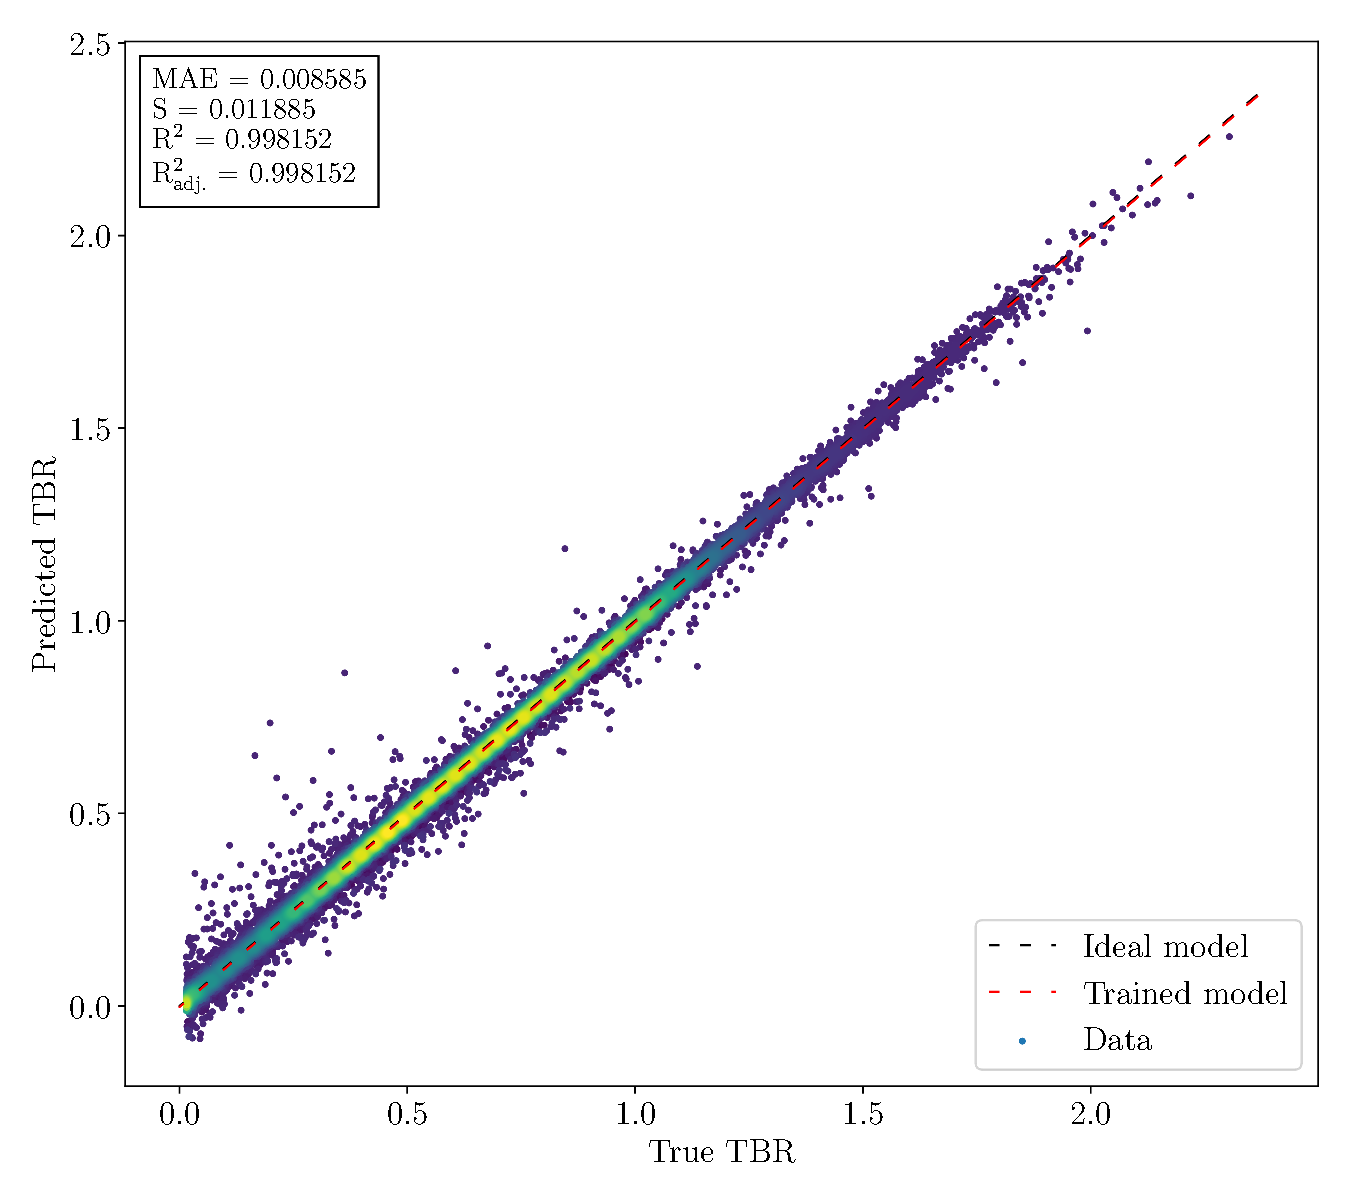
\includegraphics[width=\linewidth]{exp4_model6_rasterized}
	\end{minipage}\hfill%
	\begin{minipage}{0.5\linewidth}
		\centering
		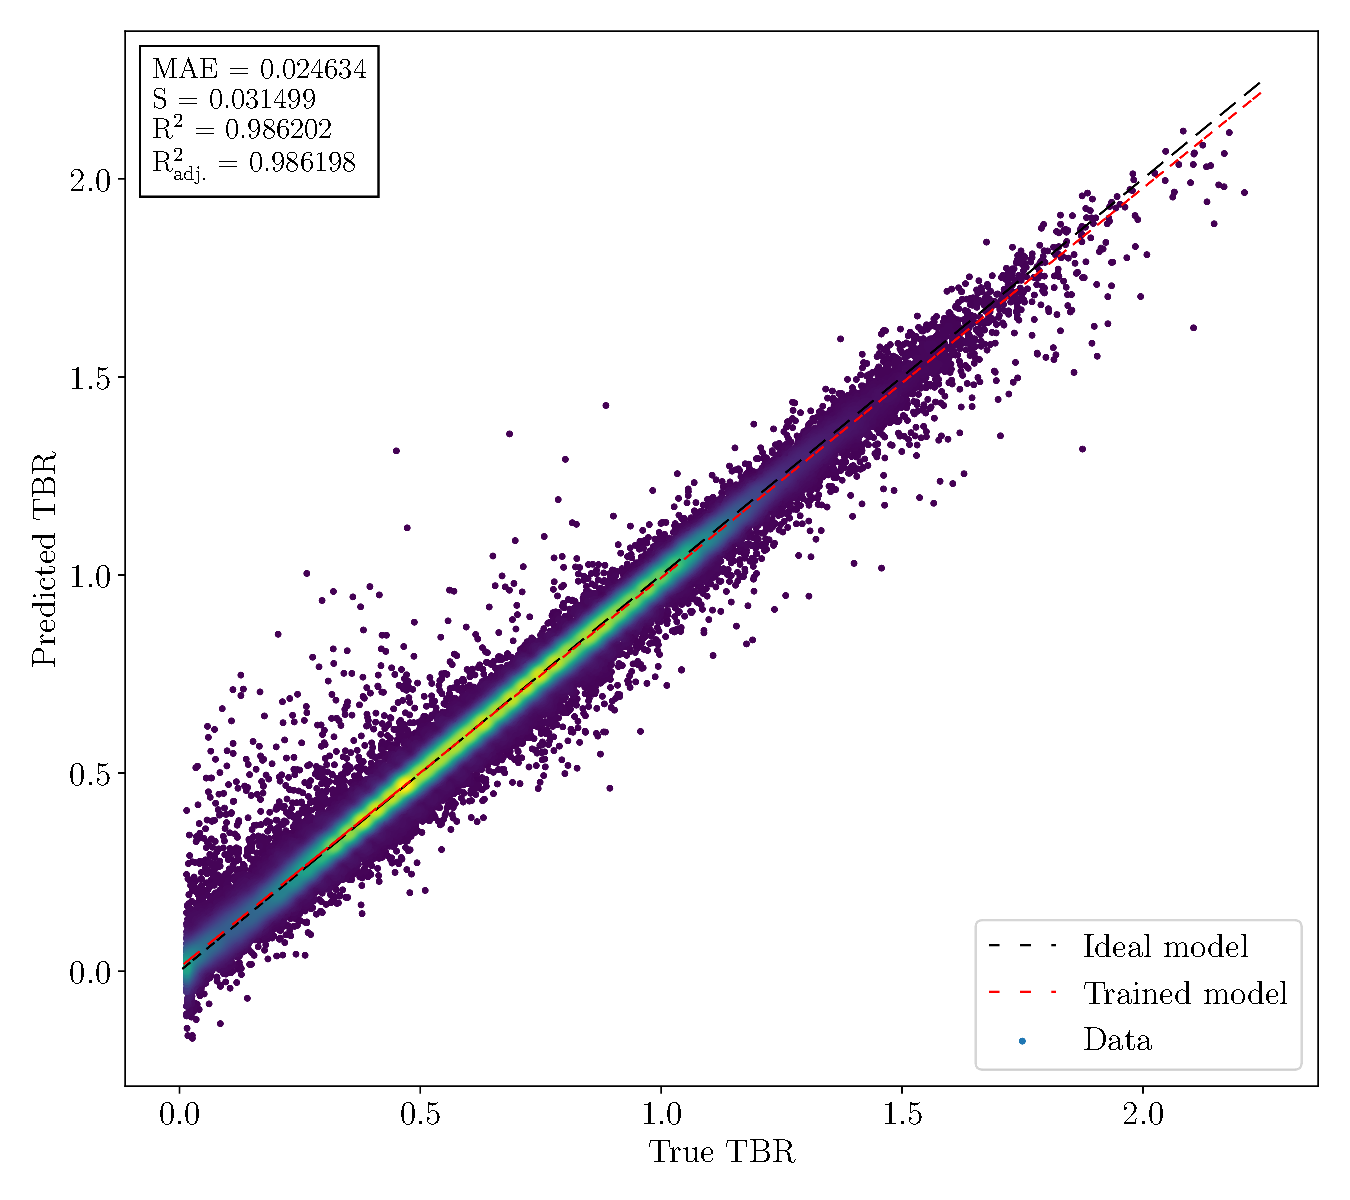
\includegraphics[width=\linewidth]{exp4_model7_rasterized}
	\end{minipage}

	\begin{minipage}{0.5\linewidth}
		\centering
		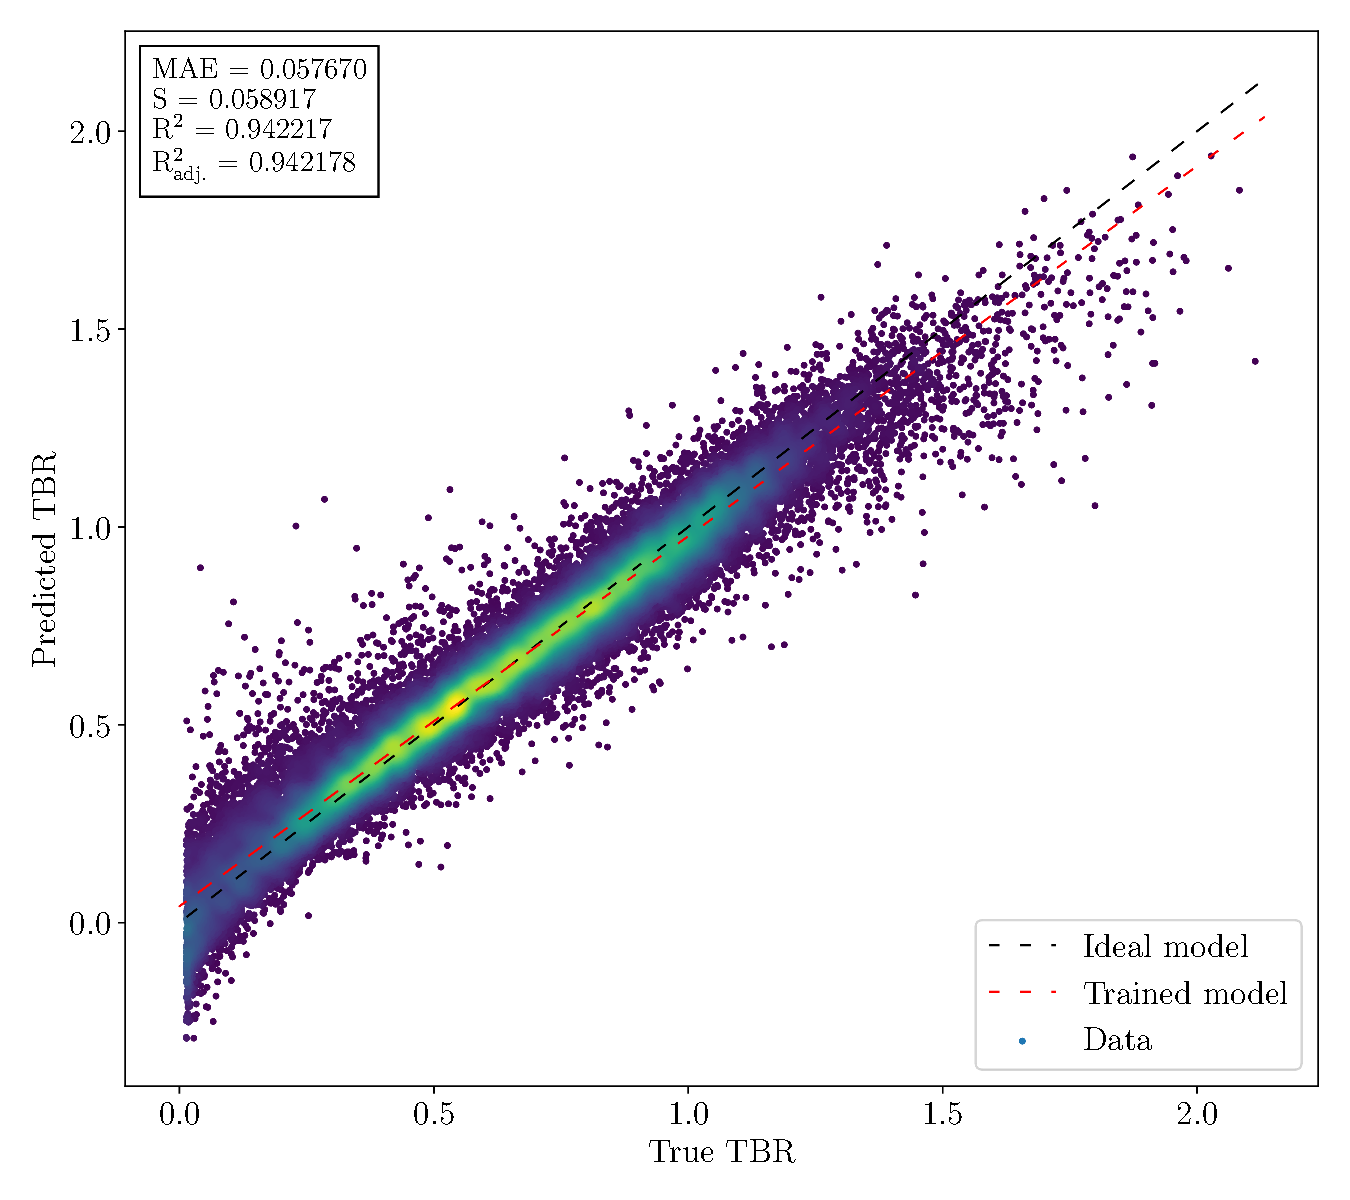
\includegraphics[width=\linewidth]{exp4_model1_rasterized}
	\end{minipage}\hfill%
	\begin{minipage}{0.5\linewidth}
		\centering
		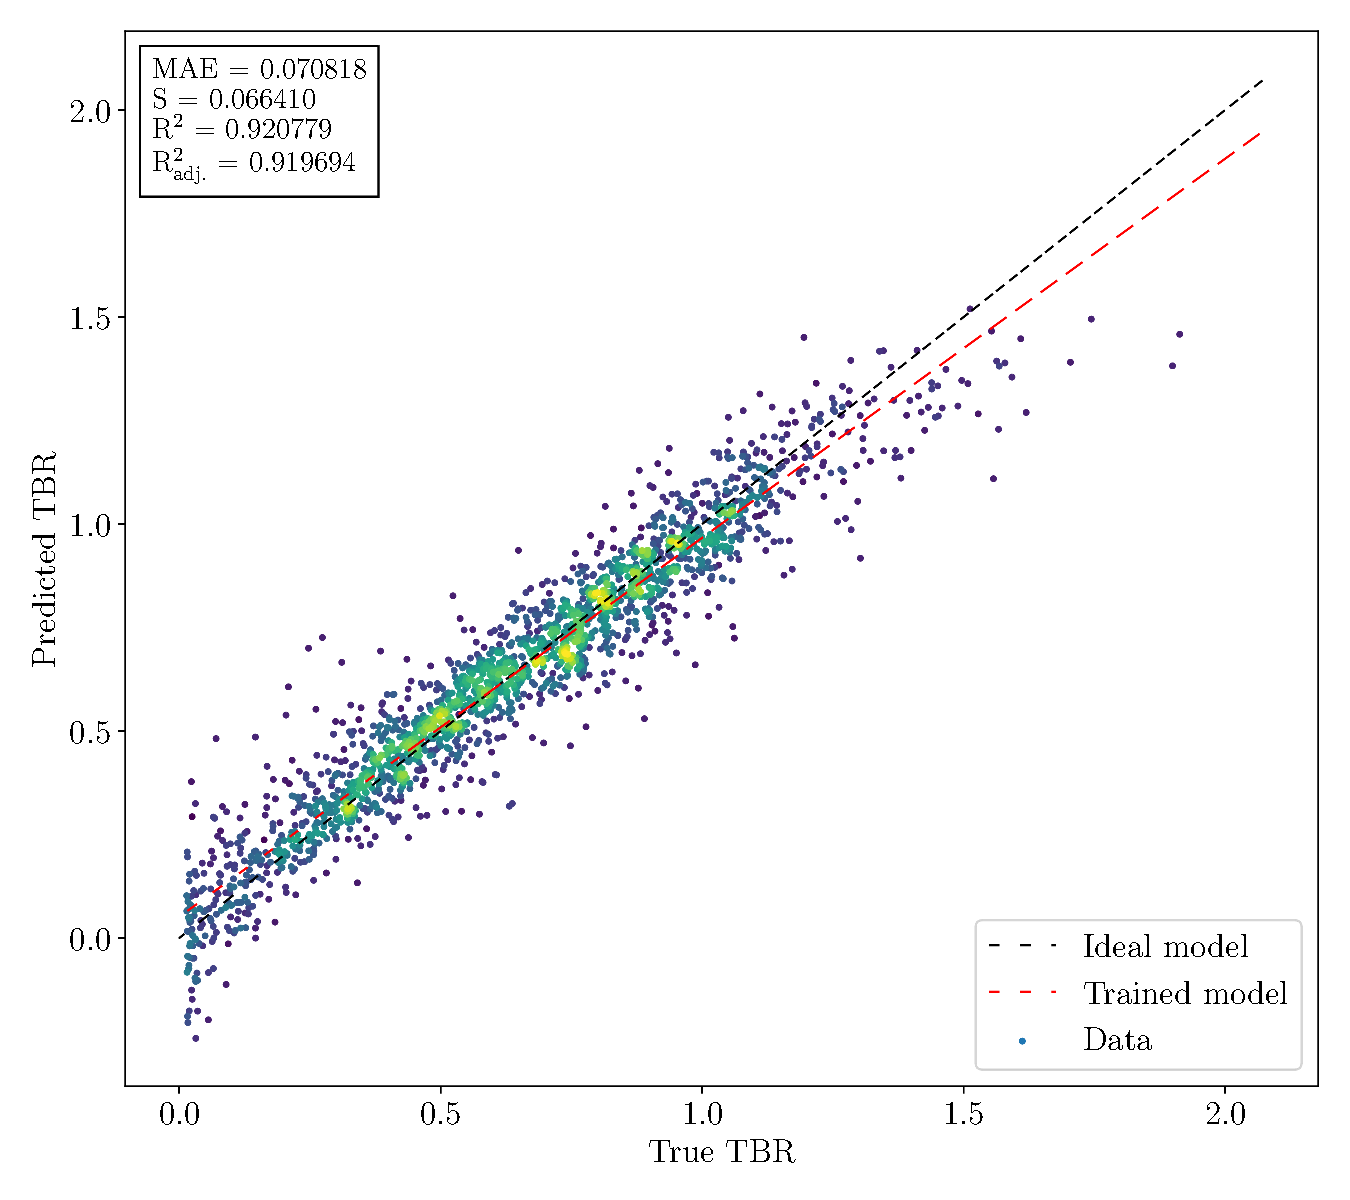
\includegraphics[width=\linewidth]{exp4_model3_rasterized}
	\end{minipage}

	\begin{minipage}{0.5\linewidth}
		\centering
		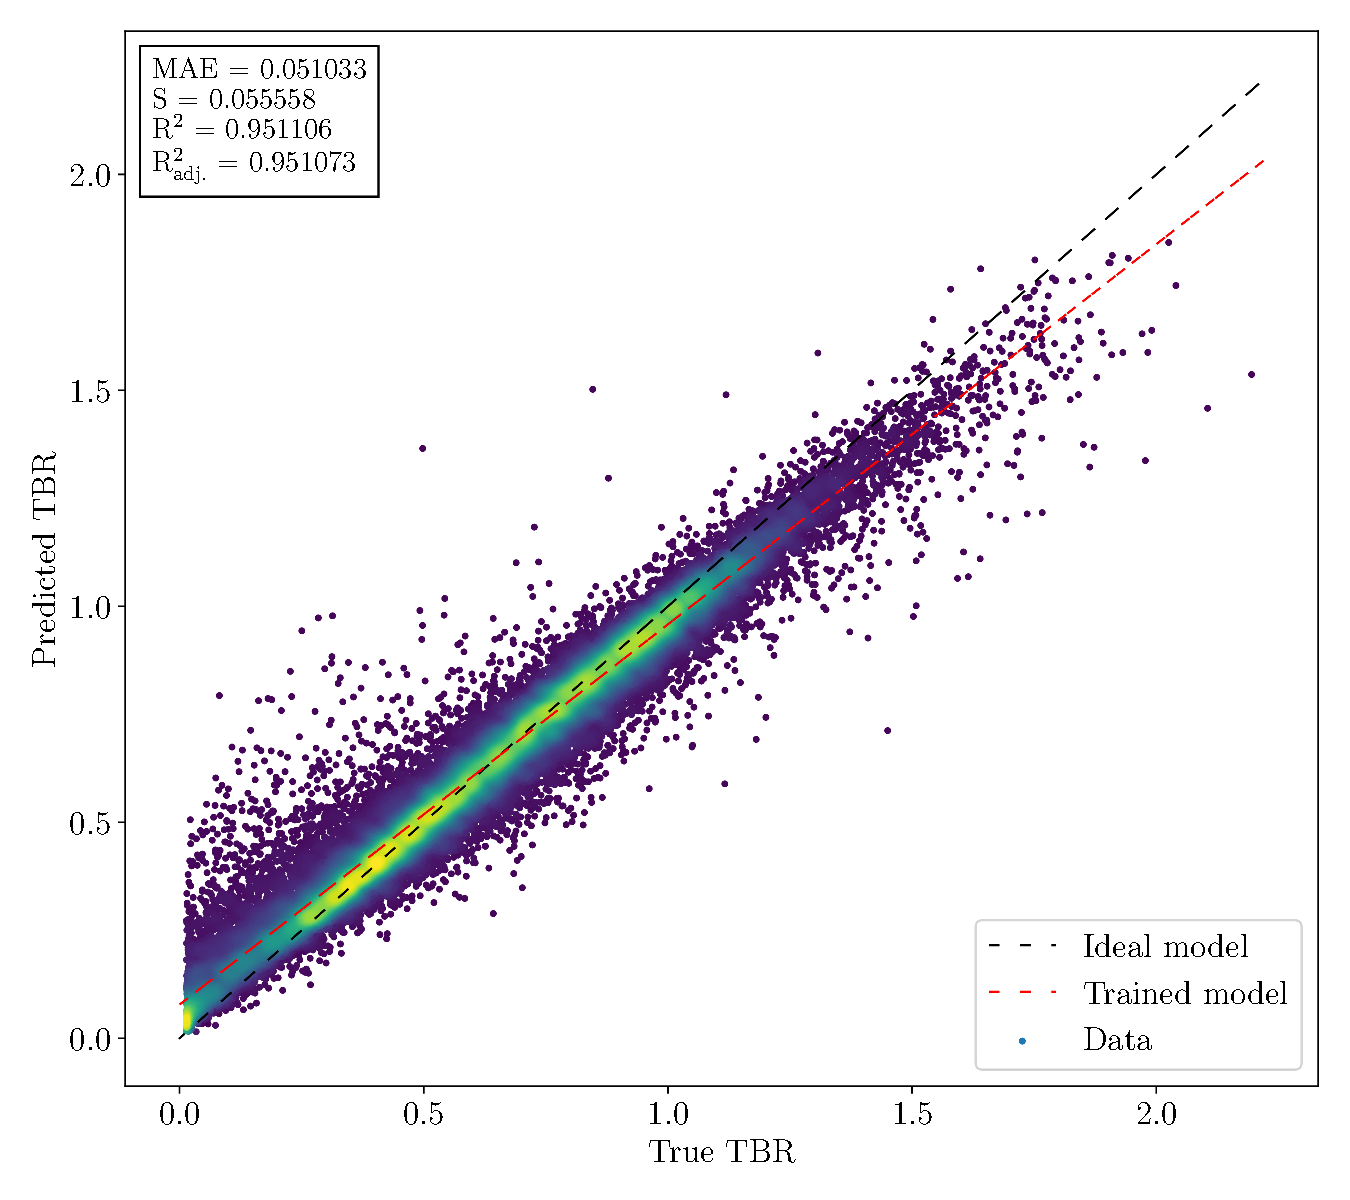
\includegraphics[width=\linewidth]{exp4_model4_rasterized}
	\end{minipage}\hfill%
	\begin{minipage}{0.5\linewidth}
		\centering
		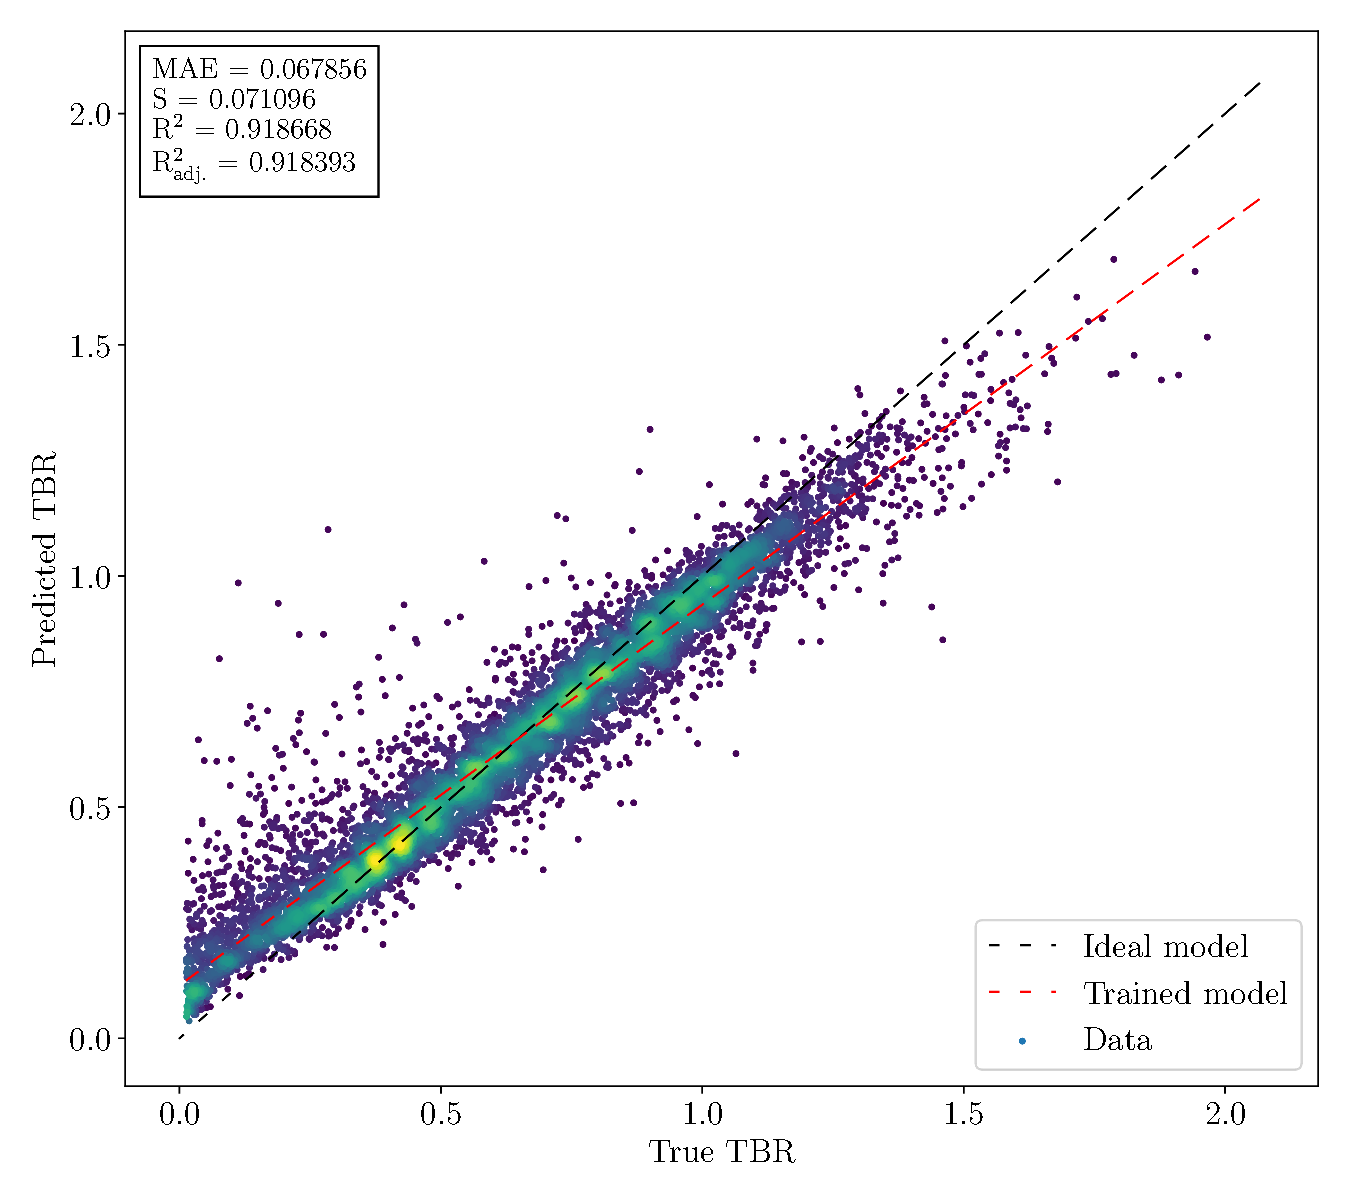
\includegraphics[width=\linewidth]{exp4_model5_rasterized}
	\end{minipage}

	\begin{minipage}{0.5\linewidth}
		\centering
		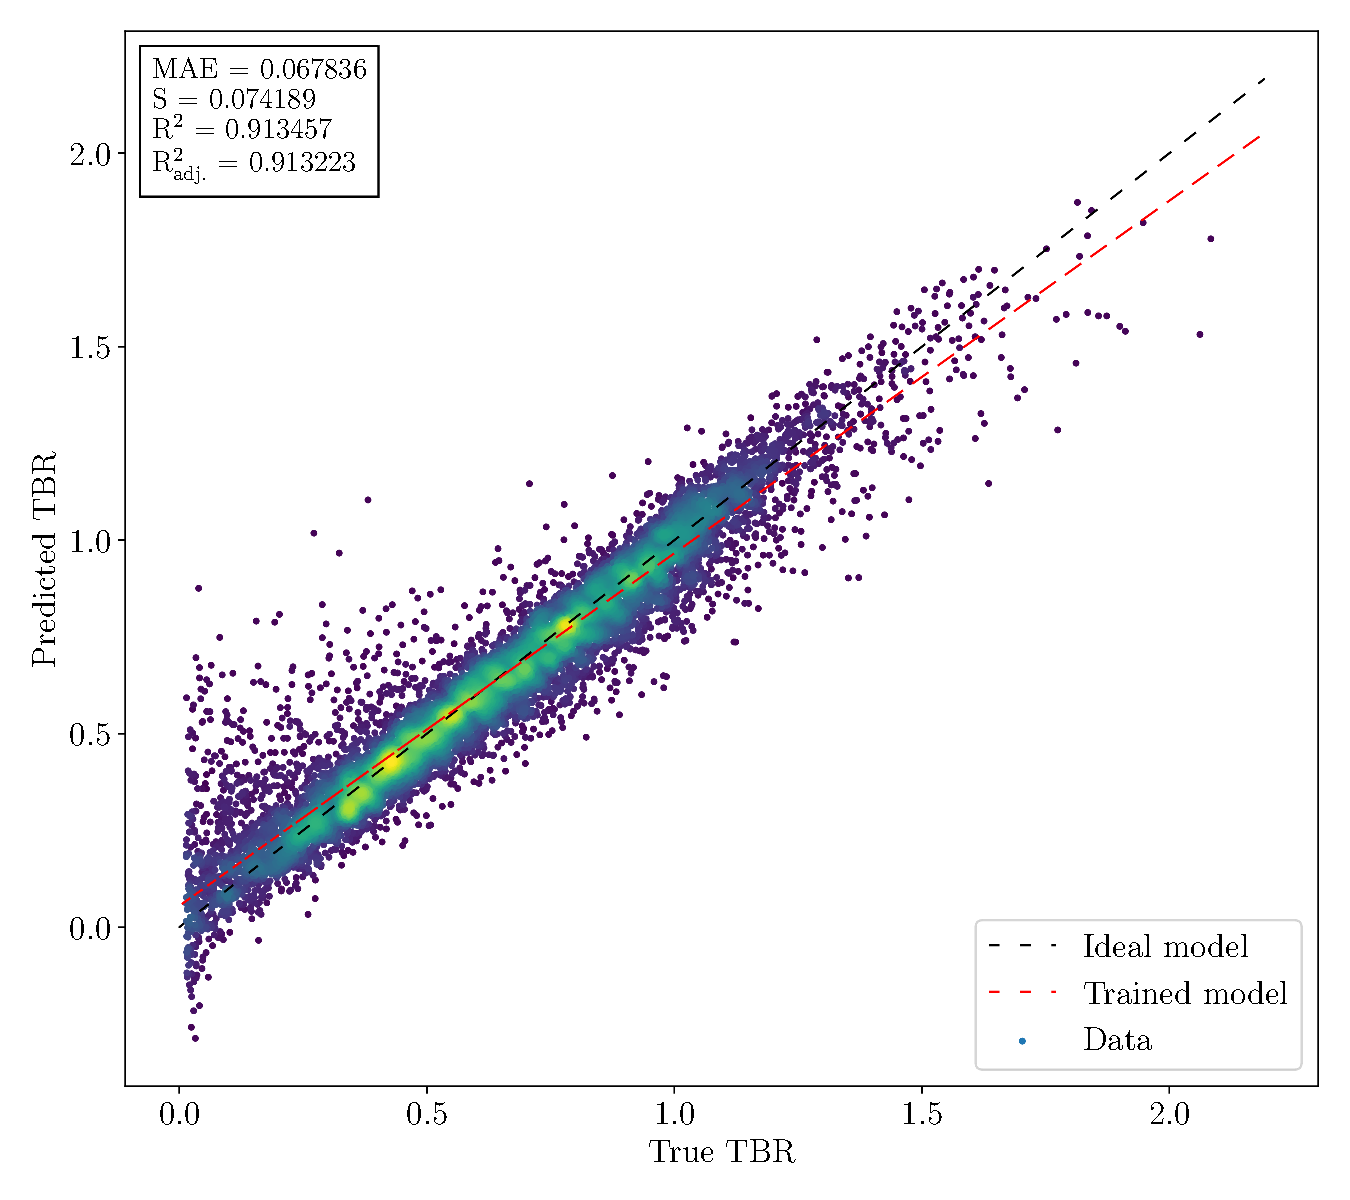
\includegraphics[width=\linewidth]{exp4_model2_rasterized}
	\end{minipage}\hfill%
	\begin{minipage}{0.5\linewidth}
		\centering
		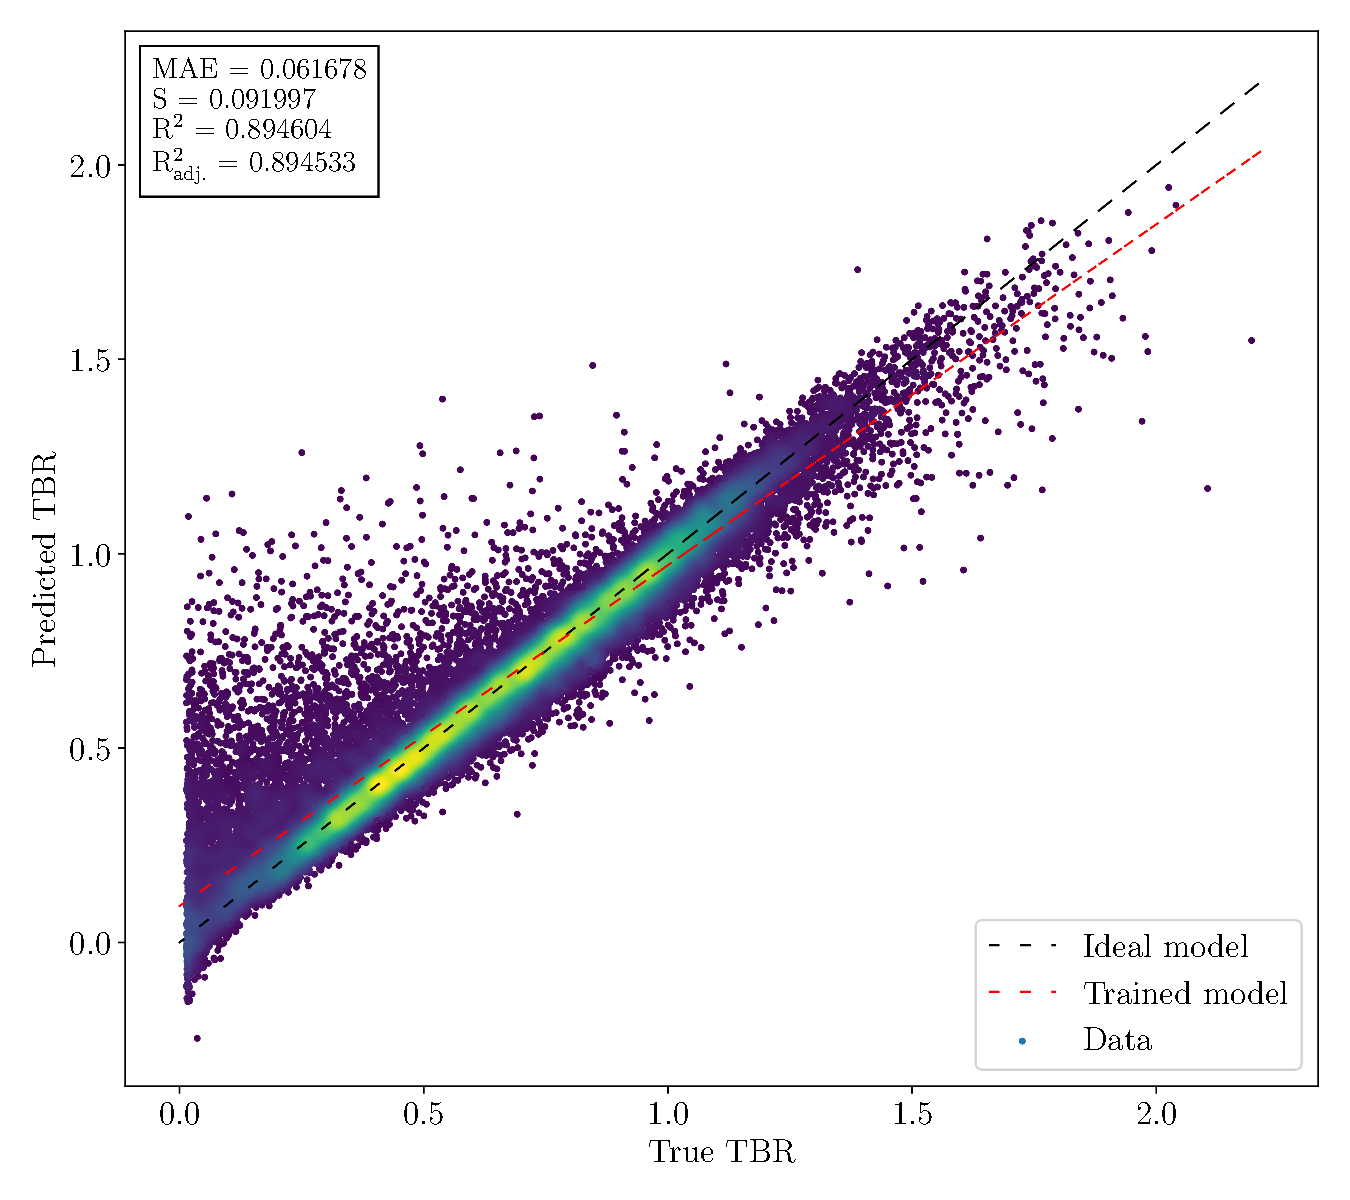
\includegraphics[width=\linewidth]{exp4_model8_rasterized}
	\end{minipage}

	\caption{Regression performance of Models~1-8 (from left to right, top to
		bottom) trained in Experiment~4, viewed
		as true vs.~predicted TBR on a test set of a selected cross-validation
		fold. Points are coloured by density.}
	\label{fig:reg-performance}
\end{figure}

Overall we found that due to their superior performance, boosted tree-based
approaches seem to be advantageous for fast surrogate modelling on relatively small training
sets (up to the order of~$10^4$). Conversely, while neural networks perform
poorly in such a setting, they dominate on larger training sets (at least of the
order of~$10^5$) both in terms of regression performance and mean prediction time.

\subsection{Adaptive Approach}\label{sec:adaptiveres}


In order to test our QASS prototype, several functional toy theories for TBR were developed as alternatives to the expensive MC model. By far the most robust of these was the following sinusoidal theory over continuous parameters $C$, with adjustable wavenumber parameter $n$:

\begin{equation}
	\text{TBR} = |C|^{-1}\sum_{i \in C} \left[1 + \sin(2\pi n (x_i - 1/2)) \right]
\end{equation}

ANNs trained on this model demonstrated similar performance to those on the expensive
MC model. QASS performance was verified by training an ANN on
the sinusoidal theory for varied quantities of initial, incremental, and MCMC
candidate samples.

An increase in initial samples with increment held constant had a strong impact
on final surrogate precision, an early confirmation of basic functionality. An
increase in MCMC candidate samples was seen to have a positive but very weak
effect on final surrogate precision, suggesting that the runtime of MCMC on each
iteration could be limited for increased efficiency. We also found that an optimum increment exists and is monotonic with initial sample quantity, above or below which models showed slower improvement on both the training and evaluation sets, and a larger minimum error on the
evaluation set. This performance distinction will be far more
significant for an expensive model such as Paramak, where the number of sample
evaluations is the primary computational bottleneck.

A plateau effect in surrogate error on the evaluation set was universal to all configurations, and initially suspected to be a residual
effect of retraining the same ANN instance without adjustment to data
normalisation. A ``Goldilocks scheme'' for checking normalisation drift was
implemented and tested, but did not affect QASS performance. Schemes in which
the ANN is periodically retrained were also discarded, as the retention of
network weights from one iteration to the next was demonstrated to greatly
benefit QASS efficiency. Further insight came from direct comparison between
QASS and a baseline scheme with uniformly random incremental samples, shown
in~\Fref{fig:qasssampling}.

\begin{figure}
	\centering
	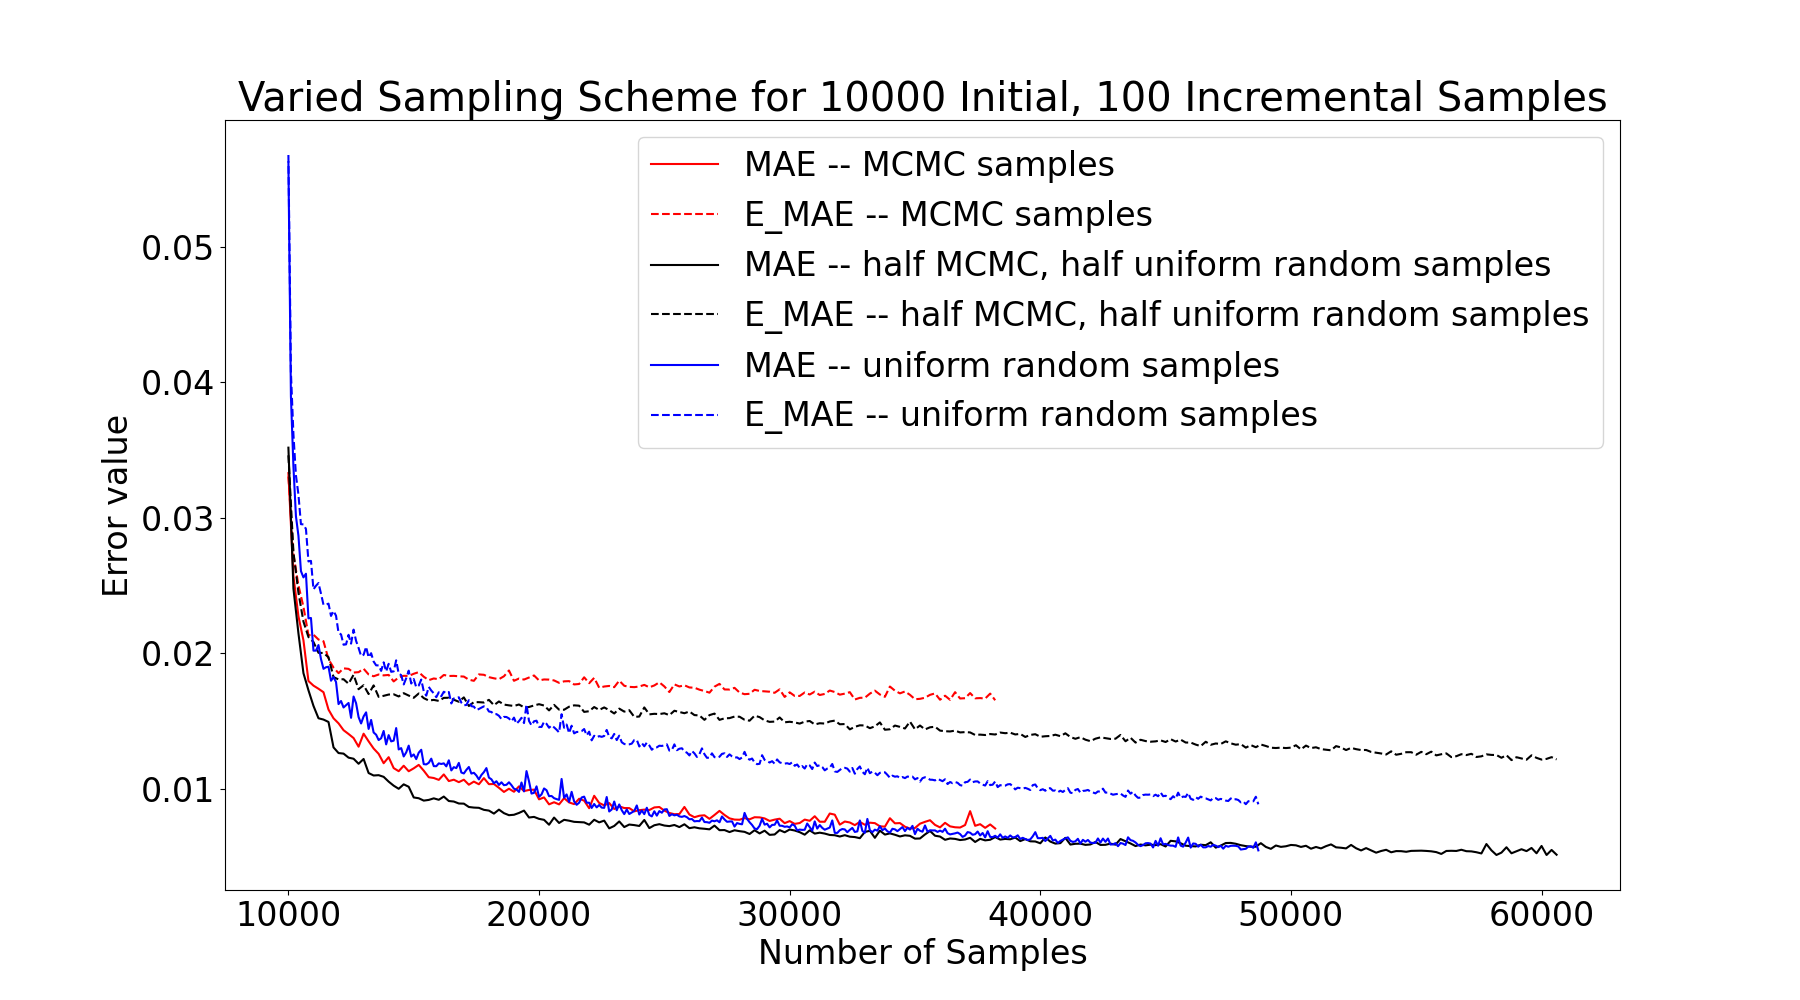
\includegraphics[width=\linewidth]{fig7_qasssampling.pdf}
	\caption{\label{fig:qasssampling}Absolute training error for QASS, baseline scheme, and mixed scheme.}
\end{figure}

\begin{figure}
	\centering
	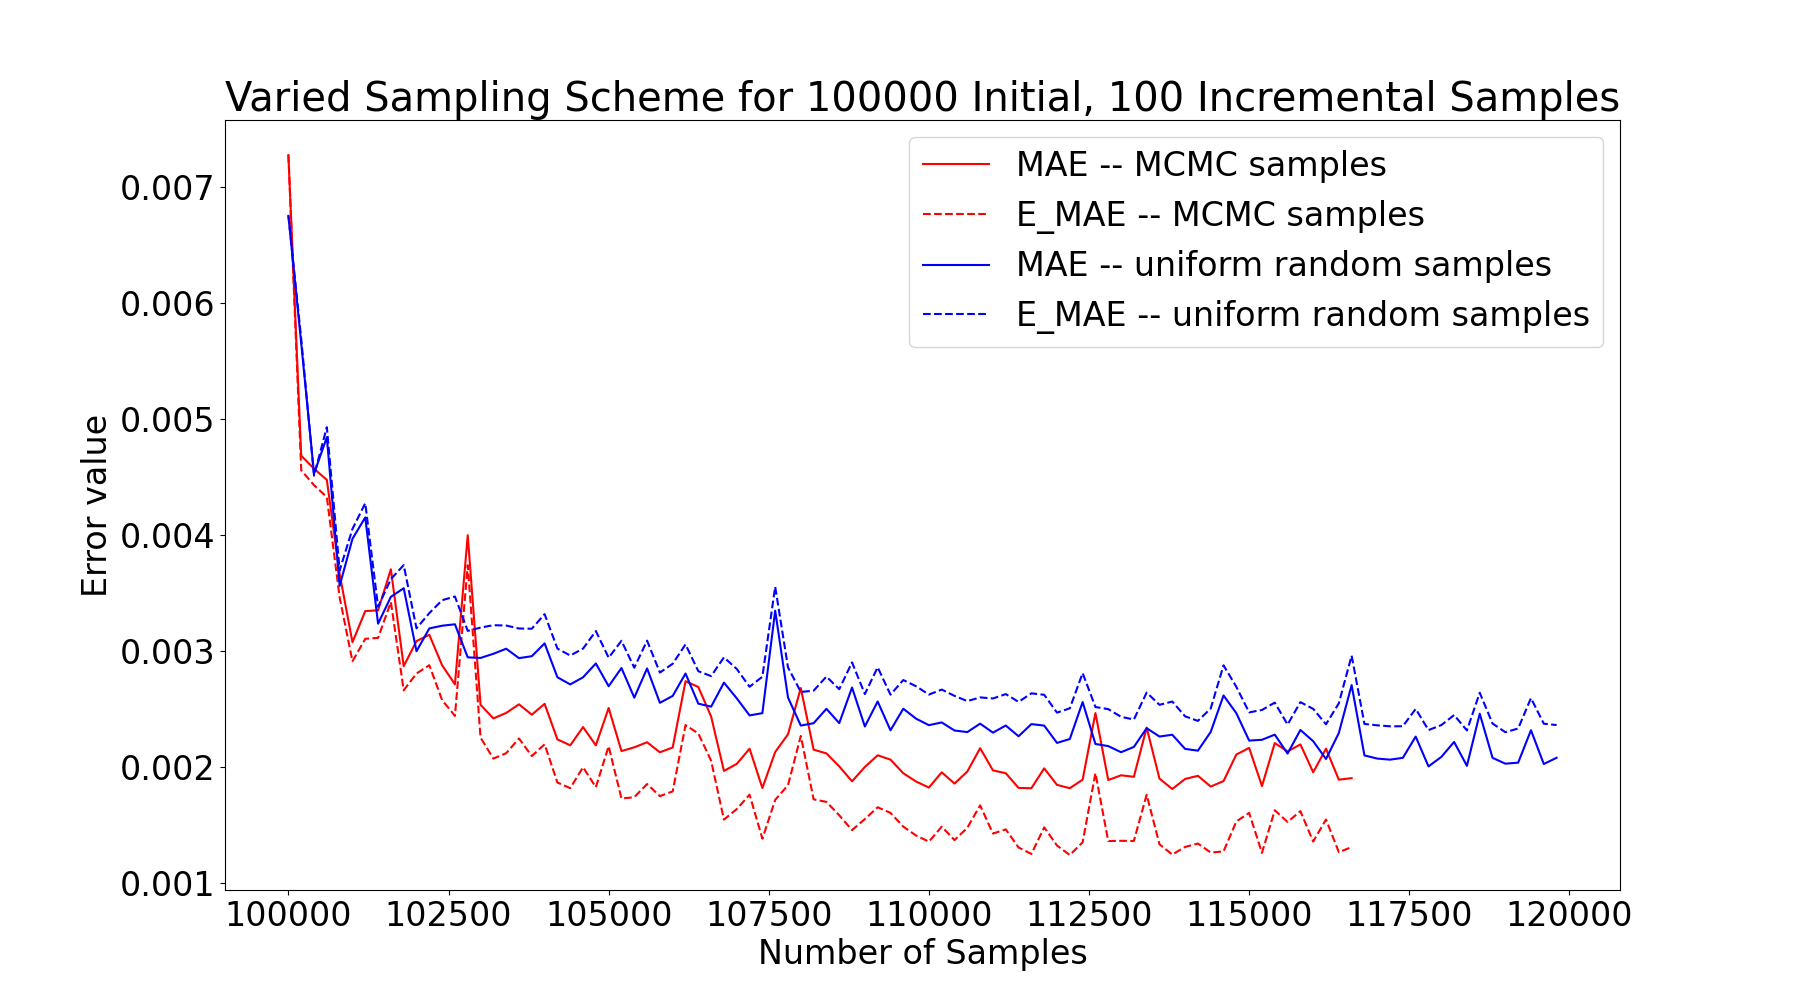
\includegraphics[width=\linewidth]{fig8_qasssampling100k.pdf}
	\caption{\label{fig:qasssampling100k}Absolute training error for QASS and baseline scheme, with 100k initial samples.}
\end{figure}

Such tests revealed that while QASS has unmatched performance on its own
adaptively-sampled training set, it is outperformed by the baseline scheme on
uniformly-random evaluation sets. We suspected that while QASS excels in
learning the most strongly peaked regions of the TBR theory, this comes at the
expense of precision in broader, smoother regions where uniformly random
sampling suffices. Therefore a mixed scheme was implemented, with half MCMC
samples and half uniformly random samples incremented on each iteration, which
is also shown in~\Fref{fig:qasssampling}. An increase in initial sample size was
observed to also resolve precision in these smooth regions of the toy theory, as
the initial samples were obtained from a uniform random distribution. As shown
in ~\Fref{fig:qasssampling100k}, with~\num{100000} initial samples it was
possible to obtain a ${\sim}40\%$ decrease in error as compared to the baseline
scheme, from 0.0025 to 0.0015 mean averaged error. Comparing at the point of
termination for QASS, this corresponds to a ${\sim}6\%$ decrease in the number
of total samples needed to train a surrogate with the same error. 




\section{Conclusion}
\label{sec:conclusion}
\begin{frame}
	\frametitle{Conclusion}

	\begin{block}{Decoupled Approach}
		\begin{itemize}
			\setlength\itemsep{0em}
			\item
				Heuristic: \alert{GBTs} for $<10^4$~samples,
				\alert{ANNs} for $\geq10^5$~samples.
			\item
				Fastest found surrogate evaluates TBR in~\SI{0.898}{\micro\second}
				with error~$\num{0.033}$. This is roughly~\alert{$8\cdot
				10^6\times$~faster} than Paramak.
			\item
				Found surrogates with comparable properties with
				\alert{$\approx$10K~samples}.
		\end{itemize}
	\end{block}

	\begin{block}{Adaptive Approach}
		\begin{itemize}
			\setlength\itemsep{0em}
			\item
				New theoretical approach \alert{QASS} developed, based on MCMC.
			\item 
				\alert{$60\%$ decrease} in evaluation MAE demonstrated.
			\item
				\alert{$6\%$ decrease} in expensive TBR samples needed.
		\end{itemize}
	\end{block}

	\begin{itemize}
		\item 
			All methods \alert{portable} $\rightarrow$ cheap approximation of any simulation.
		\item
			Article in IOP \alert{Journal of Nuclear Fusion} (pending).
		\item
			Included as a benchmark in the \alert{SciML Collaboration}.
	\end{itemize}

\end{frame}




%%%%%%%%%%%%%%%%%%%%%%%%%%%%%%%%%%%%%%%%%%%%%%%%%%%%%%%%%%%%%%%%%%%%%%%%%%%%%%%
% BACK MATTER
%%%%%%%%%%%%%%%%%%%%%%%%%%%%%%%%%%%%%%%%%%%%%%%%%%%%%%%%%%%%%%%%%%%%%%%%%%%%%%%

\section{Acknowledgements}
\label{sec:acknowledgements}
PM was supported the STFC UCL Centre for Doctoral Training in Data Intensive
Science (grant no. ST/P006736/1).\todo{Do we need any more?}


\section{References}
\label{sec:references}
\bibliography{ucl_tbr_paper}
\bibliographystyle{iopart-num}


\end{document}

